\section{The \sse Platform}\label{sec:platform}

Based on the concepts described in the previous chapter, Chipounov and his team implemented the \sse platform, an open source framework for writing custom system analysis tools.
\sse employs the theoretical concepts of selective symbolic execution by running the system under analysis in a virtual machine and treating code within the scope of interest as symbolic.
These symbolic parts are translated into an intermediate representation (LLVM IR), while irrelevant instructions are directly passed to the host for native execution.


Technical backbone of \sse are the virtual machine hypervisor QEMU \cite{qemu, qemu05}, the symbolic execution engine KLEE \cite{klee, klee08} and the LLVM compiler infrastructure \cite{llvm, llvm04}.
Figure \ref{fig:arch} gives an overview of how these technologies are integrated into the \sse platform.
The top of the picture depicts the software stack of the guest system (=the system under analysis), which is managed by QEMU.
\sse is not restricted to user land applications, but also allows inspection on deeper levels (e.g., operating system functions).


\begin{figure}
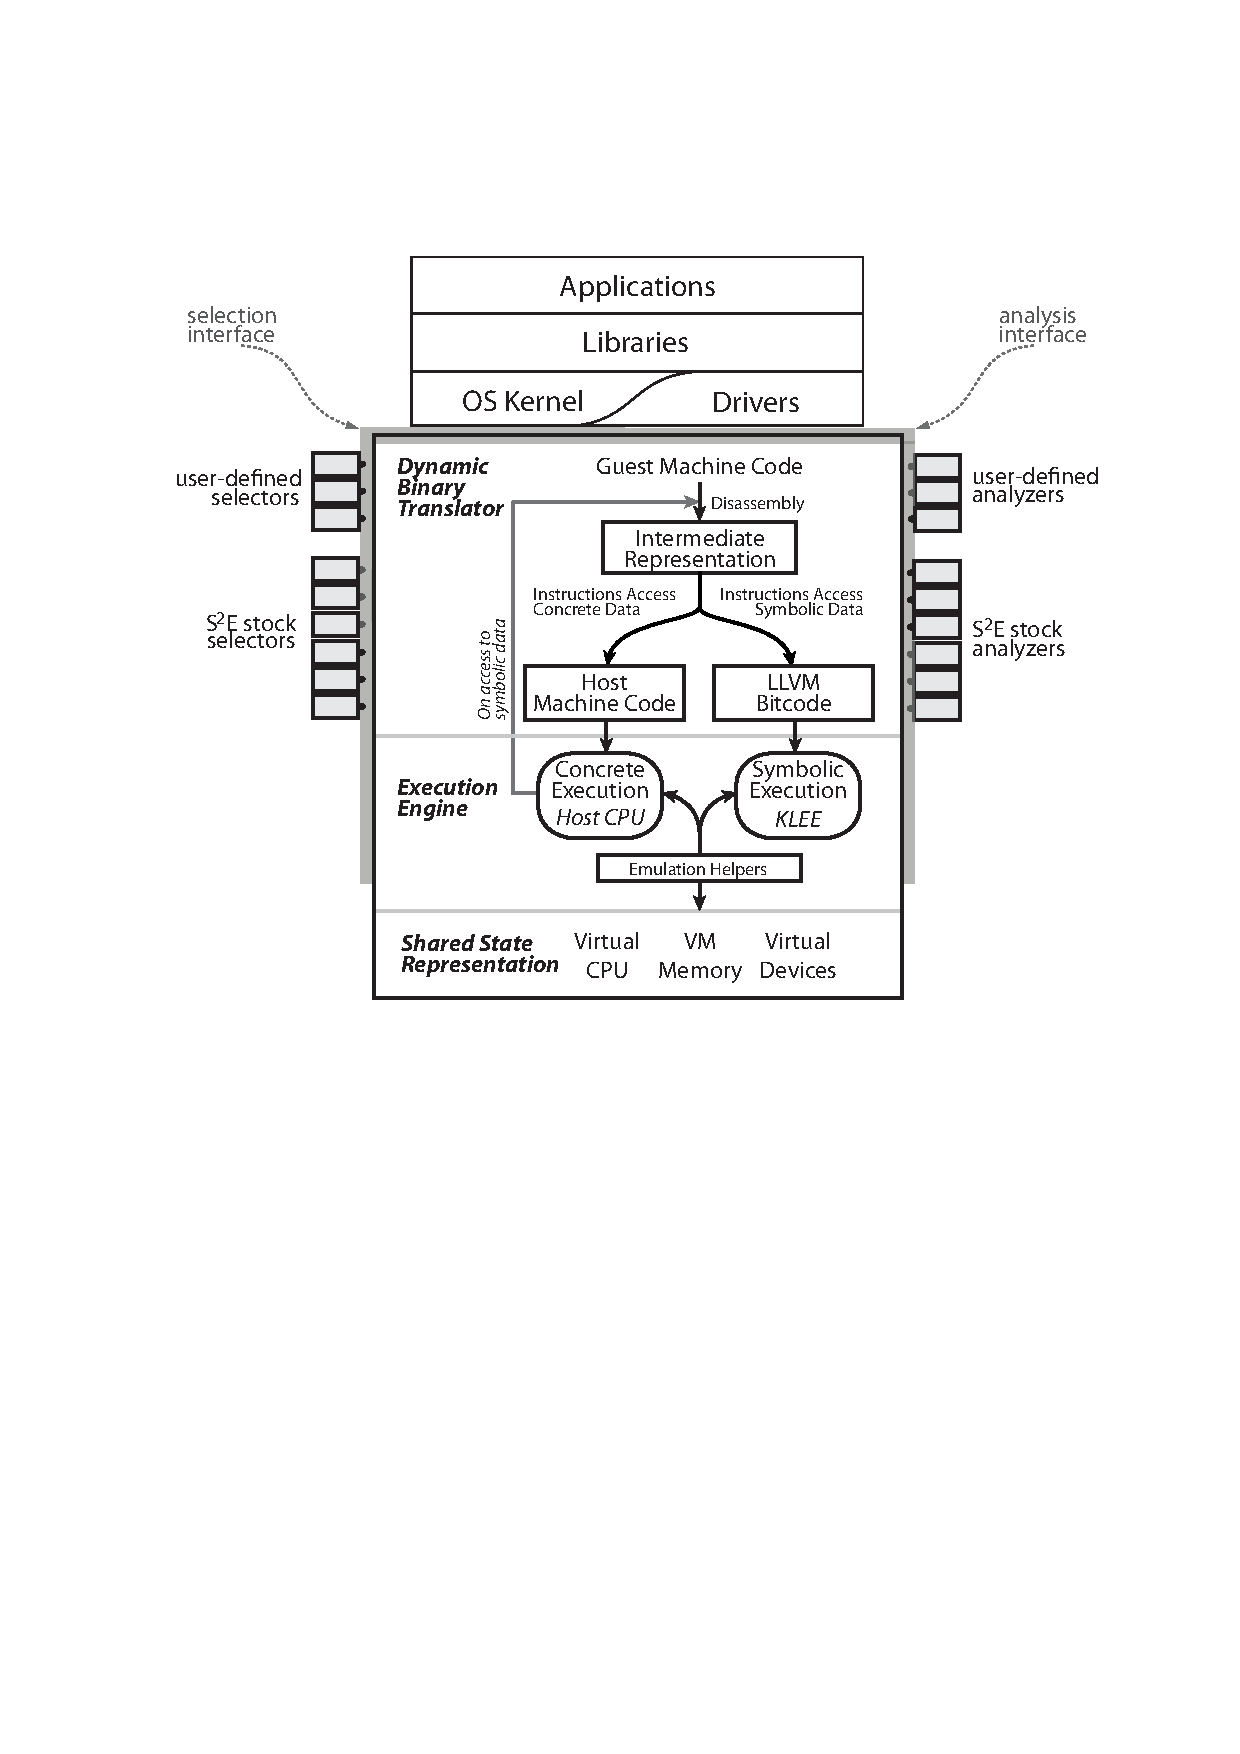
\includegraphics[width=\columnwidth]{s2e_arch}
\caption{Architecture of the \sse platform \cite{chip12s2e}}
\label{fig:arch}
\end{figure}


For easier emulation, QEMU translates machine code of the guest system into an intermediate representation, called $microoperations$.
\sse's dynamic binary translator (DBT) splits the resulting microoperations into those that need to be explored symbolically and those which may run concretely.
All concrete microoperations are directly converted into host instructions.
Symbolic expressions, on the other hand, are prepared for being executed on the KLEE engine.
This requires microoperations to be translated into the LLVM intermediate representation, called LLVM Bitcode in figure \ref{fig:arch}.

\sse's execution engine, which is an extension to QEMU's execution engine, now manages the operation of the platform.
In an endless loop it asks the DBT for new guest code.
Depending on the result, instructions can either be run straight on the host system or are fed into the KLEE symbolic execution engine.
% --- - --- - Emulation Helpers bringen?

In order to keep the mix of symbolic and concrete execution consistent, \sse stores state (VM CPU, memory, ...) centrally, by consolidating QEMU and KLEE data structures and managing them in a single machine state representation.
% - --- - - - Effizienz bringen?


Users work with \sse by writing selection and analysis plugins or by simply configuring \sse's standard plugins according to their needs.
Plugins subscribe to system-wide events (e.g., $onInstrExecution$) and can perform logging/monitoring tasks or even manipulate the system state.

Configuration usually starts with defining what parts of the system to explore symbolically.
This can for example be done with \sse's selection plugin $CodeSelector$, which restricts symbolic execution to a specified module or code region.

Standard analysis plugins allow users to find bugs ($WinBugCheck$), monitor memory ($MemoryChecker$), study performance characteristics ($PerformanceProfiler$) and much more (see \cite{chip14s2e}, p.~50).
% - ------- hier mehr?
%\todo{m?}



% ---------------------------------------------------------------- %
\iffalse
§3	The S2E Platform
		> Architektur
		> Funktionsweise
		> Selektoren + Analysatoren
\fi